\chapter{Deep Learning Modelle im Web}
Das Modell muss in einer Art und Weise für den Nutzer zugänglich gemacht werden. Das Modell welches in dieser Arbeit entwickelt wurde, kann nur Zahlen verstehen. Es muss also in erster Linie ein Encoder diese Strings in Zahlen umwandeln. Je nach Plattform wird dann die Berechnung stattfinden, welches Vorhersagt, ob die Eingabe ein Clickbait war oder nicht. 

Bevor TensorFlow.js entwickelt wurde, ließ dieses sich mittels eines Servers erfolgen. Ein HTTP-Endpunkt welches die Eingabe z.B. mittels JSON liest, kann dann im Server die Berechnung ausführen (serverseitig). Durch TensorFlow.js kann das Modell in den Browser geladen werden und zur Inferenz herangezogen werden.

In diesem Abschnitt wird zunächst die konventionelle, serverseitige Alternative Vorgstellt, im Anschluss darauf wird die in dieser Arbeit vorgeschlagene Methode des clientseitigen Deep Learnings, praktisch angewendet. Beide Methoden haben Ihre Vor- und Nachteile, diese sollen anschließend analysiert werden.

\section{Serverseitiges Deep Learning}
Um das Deep Learning auf der Seite des Servers auszuführen wird ein Server mittels Flask, welches in Python geschrieben wurde, entwickelt. Dieser Server hat nur eine Route, welches ein POST-Request aufnimmt. Dieser Request wird als JSON zugeführt. Nachdem der Server diese JSON-Information aufgenommen hat, kann er den Text in das Modell weitergeben. Da das Modell nur Zahlen versteht, ist das Encoden der Texte erforderlich. 

\begin{lstlisting}[language=Python,caption=Beispiel eines Servers für die Vorhersage von Clickbaits, label={Server}]
from flask import Flask, request
from keras.preprocessing.text import tokenizer_from_json
from keras.preprocessing.sequence import pad_sequences
from keras.models import load_model
from flask import request
import numpy as np
import json


labels = np.array(["Clickbait", "News"])
model = load_model(2model/model.h5")
with open("model/tokenizer.json") as f:
    tokenizer = tokenizer_from_json(json.load(f))


def encode(text):
    return pad_sequences(tokenizer.texts_to_sequences(text), maxlen=40)


@app.route("/predict", methods=["POST"])
def postJsonHandler():
    if request.method == "POST":
        return json.dumps({"prediction": labels[np.argmax(model.predict(encode([request.get_json()["text"]])))]})

        
if __name__ == "__main__":
    app.run()
\end{lstlisting}

Der Client kann einen HTTP-Endpunkt dafür verwenden, um die Verbindung mit dem Server und somit mit dem Modell durchzuführen.



\section{Clientseitges Deep Learning}
Dieser Abschnitt beschäftigt sich mit dem clientseitigen Deep Learning. Um TensorFlow.js praktisch anzuwenden wurde in React\footnote{React ist ein Frontend Framework für JavaScript. Es wurde von Facebook entwickelt und ist Open Source} ein Frontend entwickelt, welches vom Modell gebrauch macht.  Um Inferenz zu bilden ist ein Server nicht mehr nötig. Alleine der Zugriff auf die \enquote{model.json} Datei und die jeweiligen Gewichte reichen für diese Variante aus. Die Dateien werden auf einem Server von AWS gehostet und können in den Browser geladen werden. Das Frontent wird außerdem die gesamte TensorFlow.js Bibliothek in den Browser laden müssen. Da die gesamte Inferenz im Browser stattfindet, muss auf die Größe des Modells geachtet werden. Das in dieser Arbeit entwickelte Modell ist mit seiner gesamten Größe von 3 MB relativ klein. 

\begin{lstlisting}[language=bash,caption=Wichtigste Elemente der Benuteroberfläsche, label={OrdnerStr}]
|____src
| |____constants
| | |____constants.js
| |____hooks
| | |____index.js
| | |____useLoadVocab.js
| | |____useLoadModel.js
| |____helpers
| | |____splitText.js
| | |____index.js
| | |____tokenize.js
| |____index.js
| |____App.js
\end{lstlisting}

\section{Tokenisierung und Padding}
Unter dem Verzeichnus \enquote{helpers} befinden sich die Skripte zur Erstellung der Tokens. Der von dem User eingegebene Text muss in seine Tokens gebracht und außerdem muss die Interpunktion gefiltert werden (außer Ausrufezeichen und Fragezeichen). Ein Wort darf außerdem nicht weniger als ein Zeichen enthalten und außerdem müssen die Wörter in Kleinbuchstaben umgewandelt werden, da das \enquote{vocab.json} nur solche enthält. Im Listing~\ref{splitText} wird die Funktion dargestellt, welches den Satz, welches der Nutzer eingibt in Token umwandelt. Hier wird ein vorprogrammiertes Tokeniser\footnote{https://www.npmjs.com/package/wink-tokenizer} verwendet, welches die Tokens taggen kann. Die Tokens werden entsprechend gefiltert und und als Array zurückgegeben. Das Ergebnis dieser Prozedur muss den Tokens aus der Python Umbegung gleichen, sonst wird das Modell etwas anderes zu Gesicht bekommen, als eingegeben.

\begin{lstlisting}[language=JavaScript, caption=Die splitText Funktion, label={splitText}]
const tokenizer = require('wink-tokenizer');
const myTokenizer = tokenizer();

const splitText = (sentence) => {
  const tokens = myTokenizer.tokenize(sentence);
  const splitted = [];
  tokens.forEach((token) => {
    if (token.tag === 'number') {
      splitted.push(token.value);
    } else if (token.tag === 'word') {
      if (token.value.length >= 1) {
        splitted.push(token.value.toLowerCase());
      }
    } else if (token.tag === 'punctuation') {
      if (token.value === '?' || token.value === '!') {
        splitted.push(token.value);
      }
    }
  });

  return { splitted: splitted, splittedLen: splitted.length };
};

export default splitText;
\end{lstlisting}

Im nächsten Schritt müssen die Tokens in Zahlen umgewandelt werden. In der Python Umgebung wurde dies mit der Methode \texttt{pad\_sequences} aus der Keras-Bibliothek ausgeführt. In JavaScript gibt es keinen Ersatz für diese Methode, sodass es selbst programmiert wird. Die \texttt{tokenize}-Funktion nimmt den Text den der Client eingibt und führt diese in die \texttt{splitText}-Funktion ein. Für alle Tokens wird ein Abgleich mit der \texttt{vocab.json} erstellt und wenn ein Treffer gefunden wurde, der Index in eine Array eingeführt. Die maximale Länge wird später aus der Datei \texttt{constants.js} entnommen und beträgt in diesem Beispiel 40. Damit entsteht ein Array der Länge 40, mit \textit{n} Treffern und \textit{40-n} Nullen. Der Parameter \texttt{vocabLoading} ist ein Boolean, welches eine Aussage darüber gibt, ob die \texttt{vocab.json} lädt oder nicht, welches asynchron geladen wird, da sonst dieser Prozess den gesamten Verlauf blockieren würde. 


\begin{lstlisting}[language=JavaScript, caption=Die tokenize Funktion, label={tokenizejs}]
import splitText from './splitText';

const tokenize = (text, vocabLoading, vocab, maxLen) => {
  const { splitted } = splitText(text);
  const tokens = [];

  if (!vocabLoading) {
    splitted.forEach((element) => {
      if (vocab[element] !== undefined) {
        tokens.push(vocab[element]);
      }
    });

    while (tokens.length < maxLen) {
      tokens.push(0);
    }
  }
  return tokens.slice(0, maxLen);
};

export default tokenize;
\end{lstlisting}

\section{Laden des Modells und Vokabulars}
Die sich im Verzeichnis \enquote{hooks} befindenden Dateien \texttt{useLoadVocab} und \texttt{useLoadModel} sind sogenannte Benutzerdefinierte React Hooks \footnote{Hooks sind eine relativ neue Ergänzung in React. Mit ihnen können funktionale UI-Komponenten verwendet werden, die die herkömlichen Klassen ersetzen.}. Mit einem benutzerdefinierten Hook soll die Logik einiger Komponenten in eine wiederverwendbare Funktion extrahiert werden. Sie ist eine JavaScript-Funktion. Die \texttt{useLoadModel} und \texttt{useLoadVocab} Hooks sind sehr ähnlich. Sie fetchen aus einer Url das Modell oder das Vokabular asynchron und geben, wenn Fehler beim fetchen entstehen, einen Fehler zurück. Außerdem teilen Sie der UI mit, ob das Modell oder das Vokabular lädt. Somit wird die Logik abstrahiert und kann durch einfachen Abruf woanders im Code ausgeführt werden. Durch das Einbinden von TensorFlow.js in die UI, hat der Client vollen Zugriff auf die Klasse TensorFlow. Mit der Methode \texttt{loadLayersModel} kann ein Modell geladen werden, welches aus Ebenenen besteht, einschließlich seiner Gewichte. Die Methode \texttt{ready} gibt ein Promise zurück, welches aufgelöst wird, wenn das aktuell ausgewählte Backend initialisiert wurde. Es findet also eine \enquote{asynchrone Initialisierung} statt.


\begin{lstlisting}[language=JavaScript, caption=Das useLoadModel Hook, label={useLoadModel}]
import { useState, useEffect } from 'react';
import * as tf from '@tensorflow/tfjs';

const useLoadModel = (url) => {
  const [model, setModel] = useState();
  const [modelLoading, setModelLoading] = useState(true);
  const [modelError, setModelError] = useState('');
  
  const loadModel = async (url) => {
    try {
      const model = await tf.loadLayersModel(url);
      setModel(model);
      setModelLoading(false);
    } catch (error) {
      setModelError(error);
      setModelLoading(true);
    }
  };

  useEffect(() => {
    tf.ready().then(() => {
      loadModel(url);
    });
  }, [url]);

  return {
    model,
    setModel,
    modelLoading,
    setModelLoading,
    modelError,
    setModelError,
  };
};

export default useLoadModel;
\end{lstlisting}

\section{Die Vorhersage des Modells}
Die \texttt{predict}-Funktion wird in der Datei \texttt{App.js} aufgerufen und ist ein somit die Handler-Funktion eines Events, welches die Vorhersage ausführt, wenn gewünscht wird. Die API von TensorFlow.js bietet eine Methode Namens \texttt{tidy} welches die bereitgestellte Funktion ausführt und nach der Ausführung alle von der Funktion zugewiesenen Zwischentensoren mit Ausnahme der Funktion zurückgibt. Mit dieser Methode können Speicherleaks vermieden werden. Ein Array mit den Tokens wird in ein 2 Dimensionales Tensor umgewandelt und geht durch das Modell. Mit \texttt{dispose} wird der Tensor dann am Ende aus dem Speicher entsorgt.

\begin{lstlisting}[language=JavaScript, caption=Auszug aus der predict Funktion, label={prediJS}]
const predict = async () => {
    const predictedClass = await tf.tidy(() => {
      const tokenisation = tokenize(inputText, vocabLoading, vocab, maxLen);
      if (tokenisation.length > 0) {
        const input = tf.tensor2d(tokenisation, [1, maxLen]);
        if (!modelLoading) {
          const predictions = model.predict(input);
          return predictions.as1D().argMax();
        }
      }
    });
  };
\end{lstlisting}


\begin{figure}[H]
    \centering
    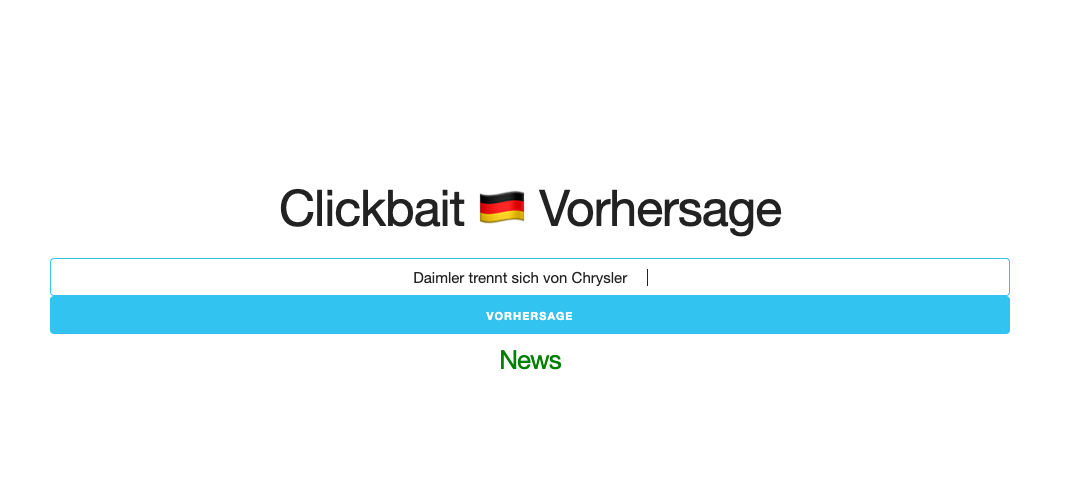
\includegraphics[width=14cm]{kapitel5/frontend.png}
    \caption[Das Frontend]{Die Benutzeroberfläsche, welches im Hintergrund mit dem Deep Learning Modell kommuniziert.}
    \label{Frontend}
\end{figure}

\section{Vergleich beider Ansätze}


In diesem Abschnitt sollen die Ansätze \enquote{serverseitiges Deep Learning} und \enquote{clientseitiges Deep Learning} verglichen werden. Beide Ansätze haben Ihre Vor- und Nachteile. Die Vorteile für das clientseitige Deep Learning sind, dass es geringe Serverkosten hat, die Inferenzlatenz geringer ist und eine Datenprivatsphäre gewährleistet ist. 

\textit{Serverkosten} spielen beim Entwerfen und Skalieren von Webdiensten eine wichtige Rolle. Häufig müssen GPU-gesützte Server bereitgestellt werden  \cite[19]{cai2020deep}. Beim clientseitigen Deep Learning muss ein kleines Modell (in diesem Beispiel 3 MB) bereitgestellt werden und daraus kann die Inferenz gebildet werden.

Ein weiterer Punkt ist die \textit{Inferenzlatenz}. Für bestimmte Arten von Anwendungen ist die Anforderung an die Latenz so hoch, dass die Deep-Learning-Modelle auf der Clientseite ausgeführt werden müssen. Alle Anwendungen, die Audio-, Bild- und Videodaten in Echtzeit enthalten, fallen in diese Kategorie. Wenn Daten erst auf ein Server geladen werden müssen um dann eine Antwort zu erhalten, steigt somit auch die Latenzzeit. Die clientseitige Inferenz behebt diese potenziellen Latenz- und Konnektivitätsprobleme, indem die Daten und die Berechnung auf dem Gerät gespeichert werden \cite[20]{cai2020deep}. Bei NLP Deep Learning Anwendungen ist fällt dieses Argument nicht so stark an, da Textdaten meistens kleiner sind, ist die Inferenzlatenz auch geringer.

\textit{Datenschutz} ist ein weiterer Vorteil des clientseitigen Deep Learnings. Das Thema Datenschutz wird heute immer wichtiger. Für bestimmte Arten von Anwendungen ist der Datenschutz eine absolute Voraussetzung. Anwendungen in Bezug auf Gesundheits- und medizinische Daten sind ein prominentes Beispiel. In vielen Ländern erlauben die Datenschutzbestimmungen für Gesundheitsinformationen nicht, dass z.B. Bilder auf einen zentralen Server übertragen werden. Eine weiteres Szenario könnten juristische Dokumente sein, die nicht auf ein drittes Server gelangen sollten \cite[20]{cai2020deep}. 

Für \textit{größere Modelle} eignet sich das clientseitige Deep Learning nicht, da es für den Nutzer nicht praktisch ist, größere Mengen an Daten (im Form eines Modells) in den Browser zu laden. Ein weiterer Vorteil für das serverseitige Deep Learning ist, dass \textit{Python} als Programmiersprache wesentlich reifer ist, als JavaScript, wenn es um Deep Learning geht. 